%=================================================%
% Section:                        	              %
%    Transport Preliminaries%
%=================================================%

\begin{center}
\section{Transport}
\label{sec:Transport}
\end{center}

%====================================================================%
% SubSection:                        	                             %
%    Transport Preliminaries: Introduction %
%====================================================================%
\aboveSubSecSkip

\subsection{Introduction}
\label{sec:Transport-Intro}

\noindent
	\indent In this chapter, the photon transport equation and material energy conservation equation are manipulated from their standard forms. The first manipulation performed is the implicit time discretization described by Fleck and Cummings. This explains the development of the Fleck factor which is used to create an effective scattering system[Fle. 1971]. The second manipulation is performed by applying the assumptions which allows for the derivation of the diffusion equation from the transport equation. Finally, the spatial discretization was developed for the diffusion equation.
			
\belowSubSecSkip

%=====================================================================%
% SubSection:                        	                              %
%     Transport Preliminaries: Radiative Transfer Preliminaries %
%=====================================================================%
\subsection{Radiative Transfer Preliminaries}
\label{sec:Transport-Radiative-Transfer-Preliminaries}

\noindent
	\indent The frequency-dependent thermal photon transport equation,
	\begin{equation}
	\label{transportEquation}
	{1\over{c}}{\partial{I(\bar{r},\nu,\bar{\Omega},t)}\over{\partial{t}}}+\bar{\Omega}\cdot\bar{\nabla}{I(\bar{r},\nu,\bar{\Omega},t)}=-\sigma(\nu)I(\bar{r},\nu,\bar{\Omega},t)+\sigma(\nu){B(\nu,T(\bar{r}))},
	\end{equation}
	\noindent describes the photon distribution in a physical system. In many problems of interest, the photon distribution is tightly coupled to the material energy balance, which is represented mathematically by,
	\begin{equation}
	\label{equationOfState}
	{1\over{c}}{\partial{E_m(T(\bar{r}))}\over{\partial{t}}}={\int\int{d\nu}{d\bar{\Omega}}\sigma(\nu)I(r,\nu,\Omega,t)-\int\int{d\nu}d\bar{\Omega}\sigma(\nu)B(\nu,T(\bar{r}))}.
	\end{equation}

	In equations \ref{transportEquation} and \ref{equationOfState} $c$ denotes the speed of light $[cm/sec]$, $\bar{r}$ denotes a location in space [cm],  $\nu$ denotes the photon frequency, $\bar{\Omega}$ denotes the solid angle of photon travel [radians], $\sigma$ denotes the opacity $[1/cm]$, $t$ is time [sec], $I(\bar{r},\nu,\bar{\Omega},t)$ is photon intensity $[photons/(cm^2*sec*steradian*eV)]$, $B(\nu,T(\bar{r}))$ is the Planck function, $E_m(T(\bar{r}))$ is the material energy density $[joules/cm^3]$, and $T(\bar{r})$ is the temperature of the background medium $[K]$.
	
	The Planck function (or Planckian),
	\begin{equation}
	\label{Planck}
	{B(\nu,T(\bar{r}))}={2h\over{c^3}}{\nu^3\over{(e^{h\nu\over{kT(\bar{r})}}-1)}},
	\end{equation}
	\noindent describes the frequency distribution of the photons being emitted from a material at temperature $T(\bar{r})$. In this function $h$ is Planck's constant $[joules*sec]$ and $k$ is Boltzmann's constant $[joules/K]$.

\belowSubSecSkip

%=====================================================================%
% SubSection:                        	                              %
%     Transport Preliminaries: Time Discretization %
%=====================================================================%
\subsection{Time Discretization}
\label{sec:Transport-Time-Discretization}

\noindent
	\indent The explicit temporal discretization of equations \ref{transportEquation} and \ref{equationOfState} can become unstable for systems that have strong absorption and remission[Gen. 2001][Fle. 1971]. This led Fleck and Cummings to develop an effective scattering which makes the equation unconditionally stable[Fle. 1971]. To derive this effective scattering, we introduce an expression for the Planck distribution function (equation \ref{Planck}); 
	\begin{equation}
	\label{newPlanck}
	{B(\nu,T(\bar{r}))}={1\over{4\pi}}b(\nu,T(\bar{r}))E_r(T(\bar{r})),
	\end{equation}
	where	
	\begin{equation}
	\label{radiationEnergyDensity}
	{E_r(T(\bar{r}))}=aT^4(\bar{r}) \nonumber
	\end{equation}
	is the equilibrium radiation energy density,
	\begin{equation}
	\label{normalizedPlanck}
	{b(\nu,T(\bar{r}))}={h\over{kT(\bar{r})}}{15\over{\pi^4}}{\left({h\nu\over{kT(\bar{r})}}\right)^3\over{(e^{h\nu\over{kT(\bar{r})}}}-1)} 
	\end{equation}
	is the normalized Planck function, and
	\begin{equation}
	\label{radiationConstant}
	{a}={8\pi^{5}k^{4}\over{15c^{3}h^{3}}} \nonumber
	\end{equation}
	is the radiation constant. Inserting these definitions into equations \ref{transportEquation} and \ref{equationOfState} yields the following new forms of the transport and energy balance equations;
	\begin{eqnarray}
	\label{Fleck1}
	&&{1\over{c}}{\partial{I(\bar{r},\nu,\bar{\Omega},t)}\over{\partial{t}}}+\bar{\Omega}\cdot\bar{\nabla}{I(\bar{r},\nu,\bar{\Omega},t)}=-\sigma(\nu)I(\bar{r},\nu,\bar{\Omega},t)\nonumber \\&&
	+{1\over{4\pi}}\sigma(\nu){b(\nu,T(\bar{r}))E_r(T(\bar{r}))}
	\end{eqnarray}
	and
	\begin{eqnarray}
	\label{Fleck2}
	&&{1\over{c}}{\partial{E_m(T(\bar{r}))}\over{\partial{t}}}={\int\int{d\nu}{d\bar{\Omega}}\sigma(\nu)I(\bar{r},\nu,\bar{\Omega},t)}\nonumber \\&&
	-{{1\over{4\pi}}\int\int{d\nu d\bar{\Omega}}{\sigma(\nu)b(\nu,T(\bar{r})){E_r(T(\bar{r}))}}}.
	\end{eqnarray}

	The Planck opacity, which is the frequency-dependent opacity averaged over the Planck distribution, is defined by;
	\begin{equation}
	\label{PlanckOpacity}
	{\sigma_p(T(\bar{r}))}={{\int^\infty_0}d\nu B(\nu,T(\bar{r}))\sigma(\nu)\over{\int^\infty_0}d\nu{B(\nu,T(\bar{r}))}}.
	\end{equation}
	Substituting equation \ref{newPlanck} into equation \ref{PlanckOpacity} and performing the integration yields;
	\begin{equation}
	\label{PlanckOpacity2}
	{\sigma_p(T(\bar{r}))}={{\int^\infty_0}d\nu b(\nu,T(\bar{r}))\sigma(\nu)}.
	\end{equation}
	
	The material energy balance (equation \ref{equationOfState}) can now be rewritten with a new expression for the source emission term($\int\int{dv}d\bar{\Omega}\sigma(v)B(v,T(\bar{r}))$). The expression for the Planck distribution function (equation \ref{newPlanck}) is inserted into equation \ref{equationOfState} and integration over all angles is performed.
	\begin{equation}
	\label{Fleck3}
	{1\over{c}}{\partial{E_m(T(\bar{r}))}\over{\partial{t}}}={\int\int{d\nu}{d\bar{\Omega}}\sigma(\nu)I(\bar{r},\nu,\bar{\Omega},t)-\sigma_p(T(\bar{r})){E_r}}
	\end{equation}
	
	The time rate of change of the material energy density can be defined in terms of the time rate of change of material temperature using the ideal gas law[Inc. 2002];
	\begin{equation}
	\label{materialEnergyDensity}
	{\partial{E_m(T(\bar{r}))}\over{\partial{t}}}={\rho(T(\bar{r})){c_v(T(\bar{r})){\partial{T(\bar{r})}\over{\partial{t}}}}}.
	\end{equation}
	In practice,  $\rho(T(\bar{r}))$ and $c_v(T(\bar{r}))$ are assumed to be constant over a time step. Equation \ref{Fleck3} can be expressed in terms of temperature by substituting in equation \ref{materialEnergyDensity}: 
	\begin{equation}
	\label{Fleck4}
	{\rho(T(\bar{r})){c_v(T(\bar{r}))}\over{c}}{\partial{T(\bar{r})}\over{\partial{t}}}={\int\int{d\nu}{d\bar{\Omega}}\sigma(\nu)I(\bar{r},\nu,\bar{\Omega},t)-\sigma_p(T(\bar{r})){aT^4(\bar{r})}}.
	\end{equation}
	This new form of the material energy balance can be discretized in time using a backwards Euler differencing:
	\begin{eqnarray}
	\label{Fleck5}
	&&{\rho(T(\bar{r})){c_v(T(\bar{r}))}\over{c}}{{T_{t+1}(\bar{r})-T_t(\bar{r})}\over{\Delta{t}}}={\int\int{d\nu}{d\bar{\Omega}}\sigma(\nu)I_{t+1}(\bar{r},\nu,\bar{\Omega},t)}\nonumber \\&& -{\sigma_p(T(\bar{r})){aT_{t+1}^4(\bar{r})}}.
	\end{eqnarray}
	The $T^4_{t+1}(\bar{r})$ on the right hand side makes this equation non-linear. To treat this non-linearity, $T^4_{t+1}(\bar{r})$ is expanded about $T_t(\bar{r})$ resulting in the following expression;
%	\begin{equation}
%	\label{tempExp1}
%	{T^4_{t+1}}=B(T_{t+1})
%	\end{equation}
%	\begin{equation}
%	\label{tempExp2}
%	B(T_{t+1})=B(T_t)+(T_{t+1}-T_t){dB(T_t)\over{dt}}+O({\Delta{T}}^2)
%	\end{equation}
%	\begin{equation}
%	\label{tempExp3}
%	{dB(T_t)\over{dt}}=4T_t^3
%	\end{equation}
	\begin{equation}
	\label{tempExp4}
	T_{t+1}^4(\bar{r})=T_t^4(\bar{r})+(T_{t+1}(\bar{r})-T_t(\bar{r}))4T^3_t(\bar{r}).
	\end{equation}

	The temperature change over the time step ${(T_{t+1}(\bar{r})-T_t(\bar{r}))}$ is obtained by substituting equation \ref{tempExp4} into the material energy balance equation (equation \ref{Fleck5}).
%	\begin{eqnarray}
%	\label{Fleck6}
%	&&{\rho{c_v}\over{c}}{{T_{t+1}-T_t}\over{\Delta{t}}}=\nonumber \\&& {\int\int{d\nu}{d\Omega}\sigma(\nu)I_{t+1}(r,\nu,\Omega,t)-\sigma_p{a(T_t^4+(T_{t+1}-T_t)4T^3_t)}},
%	\end{eqnarray}
%	and,
	% \begin{eqnarray}
	% \label{Fleck7}
	% &&{T_{t+1}-T_t}=\nonumber \\&&  {{\Delta{t}c}\over{\rho{c_v}}}\left({\int\int{dv}{d\Omega}\sigma(v)I_{t+1}(r,v,\Omega,t)-\sigma_p{aT_t^4}}\right)\nonu% mber \\&& -(T_{t+1}-T_t){\Delta{t}c\sigma_p4aT^3_t\over{\rho{c_v}}}
	% \end{eqnarray}
	% \begin{eqnarray}
	% \label{Fleck7}
	% &&{T_{t+1}-T_t}\left(1+{\Delta{t}c\sigma_p4aT^3_t\over{\rho{c_v}}}\right)=\nonumber \\&& {{\Delta{t}c}\over{\rho{c_v}}}\left({\int\int{dv}{d\Omega}\sigma(v)I_{t+1}(r,v,\Omega,t)-\sigma_p{aT_t^4}}\right)
	% \end{eqnarray}
	\begin{eqnarray}
	\label{Fleck8}
	&&{T_{t+1}(\bar{r})-T_t(\bar{r})}= \nonumber \\&& {{{\Delta{t}c}\over{\rho(T(\bar{r})){c_v(T(\bar{r}))}}}\left({\int\int{d\nu}{d\bar{\Omega}}\sigma(\nu)I_{t+1}(\bar{r},\nu,\bar{\Omega},t)-\sigma_p(T(\bar{r})){aT_t^4(\bar{r})}}\right)\over{\left(1+{\Delta{t}c\sigma_p(T(\bar{r}))4aT^3_t(\bar{r})\over{\rho(T(\bar{r})){c_v(T(\bar{r}))}}}\right)}}.
	\end{eqnarray}
	The Fleck factor, which can be described as the probability that an absorbed photon will not be reemitted during the current time step,  is defined as
	\begin{equation}
	\label{FleckFactor}
	f(T(\bar{r}))={1\over{\left(1+{\Delta{t}c\sigma_p(T(\bar{r}))4aT^3_t(\bar{r})\over{\rho(T(\bar{r})){c_v(T(\bar{r}))}}}\right)}}.
	\end{equation}
	The temperature change over the timestep can then be written as
% 	\begin{equation}
% 	\label{Fleck9}
% 	{T_{t+1}-T_t}={{{\Delta{t}c}\over{\rho{c_v}}}\left({\int\int{dv}{d\Omega}\sigma(v)I_{t+1}(r,v,\Omega,t)-\sigma_p{aT_t^4}}\right)f},
% 	\end{equation}
% 	which also implies that
	\begin{eqnarray}
	\label{Fleck10}
	&&{\rho(T(\bar{r})){c_v(T(\bar{r}))}\over{c}}{{T_{t+1}(\bar{r})-T_t(\bar{r})}\over{\Delta{t}}}=\nonumber \\&& {\left({\int\int{dv}{d\bar{\Omega}}\sigma(v)I_{t+1}(\bar{r},v,\bar{\Omega},t)-\sigma_p(T(\bar{r})){aT_t^4(\bar{r})}}\right)f(T(\bar{r}))},
	\end{eqnarray}
	or
	\begin{eqnarray}
	\label{Fleck11}
	&&{1\over{c}}{\Delta{E_m(T(\bar{r}))}\over{\Delta{t}}}={\int\int{dv}{d\bar{\Omega}}I_{t+1}(\bar{r},v,\bar{\Omega},t)\sigma(v)f(T(\bar{r}))}\nonumber \\&&
	-{\sigma_p(T(\bar{r}))f(T(\bar{r})){aT_t^4(\bar{r})}}.
	\end{eqnarray}
	
	A similar non-linearity exists in equation \ref{Fleck1} when the system is discretized in time using backward Euler differencing. We again use equation \ref{tempExp4} to write;
	\begin{eqnarray}
	\label{Fleck12}
	&&{1\over{c}}{\Delta{I(\bar{r},\nu,\bar{\Omega})}\over{\Delta{t}}}+\bar{\Omega}\cdot\bar{\nabla}{I_{t+1}(\bar{r},\nu,\bar{\Omega})}= -\sigma(\nu)I_{t+1}(\bar{r},\nu,\bar{\Omega})+\nonumber \\&& {1\over{4\pi}}\sigma(\nu){b(\nu,T(\bar{r}))a\left(T_t^4(\bar{r})+(T_{t+1}(\bar{r})-T_t(\bar{r}))4T^3_t(\bar{r})\right)}.
	\end{eqnarray}
	Substituting in the expression for the temperature change (equation \ref{Fleck8}) and performing some algebra, the transport equation can be rewritten to include a new effective scattering term.
	\begin{eqnarray}
	\label{Fleck13}
	& &{1\over{c}}{\Delta{I(\bar{r},\nu,\bar{\Omega})}\over{\Delta{t}}} + \bar{\Omega}\cdot\bar{\nabla}{I_{t+1}(\bar{r},\nu,\bar{\Omega})}=\nonumber \\& & -I_{t+1}(\bar{r},\nu,\bar{\Omega})\sigma(\nu)+{1\over{4\pi}}b(\nu,T(\bar{r}))\sigma(\nu)f(T(\bar{r}))aT_t^4(\bar{r})\nonumber \\& & +{1\over{4\pi}}{\sigma(\nu)b(\nu,T(\bar{r}))\over{\sigma_p(T(\bar{r}))}}{\int\int{d\nu}{d\bar{\Omega}}I_{t+1}(\bar{r},\nu,\bar{\Omega})\sigma(\nu)(1-f(T(\bar{r})))}
	\end{eqnarray}
	The effective absorption opacity and scattering opacity are represented by ${\sigma(\nu){f(T(\bar{r}))}}$ and ${\sigma(\nu)(1-{f(T(\bar{r}))}})$ respectively.  The final time-discretized transport and energy balance equations, in their unconditionally stable forms, are written as
	\begin{eqnarray}
	\label{finalTransport}
	& &{1\over{c}}{\Delta{I(\bar{r},\nu,\bar{\Omega})}\over{\Delta{t}}} + \bar{\Omega}\cdot\bar{\nabla}{I_{t+1}(\bar{r},\nu,\bar{\Omega})}=\nonumber \\& & -I_{t+1}(\bar{r},\nu,\bar{\Omega})\sigma(\nu)+{1\over{4\pi}}b(\nu,T(\bar{r})\sigma_a(\nu) aT_t^4(\bar{r})\nonumber \\& & +{1\over{4\pi}}{\sigma(\nu)b(\nu,T(\bar{r}))\over{\sigma_p(T(\bar{r}))}}{\int\int{d\nu}{d\bar{\Omega}}I_{t+1}(\bar{r},\nu,\bar{\Omega})\sigma_s(\nu)}
	\end{eqnarray}
	and	
	\begin{eqnarray}
	\label{finalEqState}
	&&{1\over{c}}{\Delta{E_m(T(\bar{r}))}\over{\Delta{t}}}={\int\int{d\nu}{d\bar{\Omega}}I_{t+1}(\bar{r},\nu,\bar{\Omega})\sigma(\nu)f(T(\bar{r}))}\nonumber \\&& 
	-{\sigma_p(T(\bar{r}))f(T(\bar{r})){aT_t^4(\bar{r})}}
	\end{eqnarray}
	respectively.
	
\belowSubSecSkip

%=====================================================================%
% SubSection:                        	                              %
%     Transport Preliminaries: Diffusion Approximation %
%=====================================================================%
\subsection{Diffusion Approximation}
\label{sec:Transport-Diffusion-Approximation}

\noindent
	\indent The Monte Carlo technique applied to the solution of the implicit transport equation, Implicit Monte Carlo (IMC), has been used to solve many problems of interest in high energy density physics. However, IMC can be very computationally expensive in optically thick, highly ``scattering'' (absorption-reemission) regions. This has prompted researchers to develop {\it hybrid} methods that couple the diffusion equation in optically thick highly scattering regions to the transport equation in thin regions. To derive the diffusion equation from the transport equation, it is first necessary to integrate equation \ref{finalTransport} over all angles: 
	\begin{eqnarray}
	\label{diffusion1}
	& &\int{d\bar{\Omega}}{1\over{c}}{\Delta{I(\bar{r},\nu,\bar{\Omega})}\over{\Delta{t}}} + \int{d\bar{\Omega}}\bar{\Omega}\cdot\bar{\nabla}{I_{t+1}(\bar{r},\nu,\bar{\Omega})}=\nonumber \\& & -\int{d\bar{\Omega}}I_{t+1}(\bar{r},\nu,\bar{\Omega})\sigma(v)+{1\over{4\pi}}\int{d\bar{\Omega}}\left[b(\nu,T(\bar{r}))\sigma_a(\nu) aT_t^4(\bar{r})\right]\nonumber \\& & +{1\over{4\pi}}\int{d\bar{\Omega}}\left[{\sigma(\nu)b(\nu,T(\bar{r}))\over{\sigma_p(T(\bar{r}))}}{\int\int{d\nu}{d\bar{\Omega}}I_{t+1}(\bar{r},\nu,\bar{\Omega})\sigma_s(\nu)}\right]
	\end{eqnarray}
	
	The photon energy density $(E)$ and flux $(F)$ are defined by[Gen. 2001]
	\begin{equation}
	E(r,\nu)=\int{d\bar{\Omega}}I(\bar{r},\nu,\bar{\Omega})
	\end{equation}
	and
	\begin{equation}
	F(r,\nu)=\int{d\bar{\Omega}}\bar{\Omega}\cdot{I(\bar{r},\nu,\bar{\Omega})}.
	\end{equation}
	Inserting these equations definitions and $4\pi=\int{d\bar{\Omega}}$ yields:
	\begin{eqnarray}
	\label{finalDiffusion}
	& &{1\over{c}}{\Delta{E(\bar{r},\nu)}\over{\Delta{t}}} + \bar{\nabla}\cdot{F_{t+1}(\bar{r},\nu)}=\nonumber \\& & -E_{t+1}(\bar{r},\nu)\sigma(\nu)+{b(\nu,T(\bar{r}))}\sigma_a(\nu) aT_t^4(\bar{r})\nonumber \\& & +{\sigma(\nu)b(\nu,T(\bar{r}))\over{\sigma_p(T(\bar{r}))}}{\int{d\nu}E_{t+1}(\bar{r},\nu)\sigma_s(\nu)}
	\end{eqnarray}
	and
	\begin{equation}
	\label{EqState}
	{1\over{c}}{\Delta{E_m(T(\bar{r}))}\over{\Delta{t}}}=\int{d\nu}E_{t+1}(\bar{r},\nu)\sigma(\nu)f(T(\bar{r}))-\sigma_p(T(\bar{r}))f(T(\bar{r})){aT_t^4(\bar{r})}.
	\end{equation}
	
	A relationship between the flux and energy density (Fick's law)[Gen. 2001] can derived by assuming that the photon intensity is linearly anisotropic ($P_1$ approximation) and if the temporal derivative of the flux is small[Dud. 1976]. 
	\begin{equation}
	\label{FicksLaw}
	F(\bar{r},\nu)=-D(\nu)\bar{\nabla}{E(\bar{r},\nu)},  
	\end{equation}
	where D is the diffusion coefficient,
	\begin{equation}
	\label{DiffusionCoefficent}
	D(\nu)={1\over{3\sigma(\nu)}}.
	\end{equation}
	This diffusion coefficient is derived under the assumption that the system has isotropic scattering. It should be noted that without a ``flux limiter'' it is possible for this method to allow particles to transport faster then the speed of light. This is an unphysical behavior that can cause wave fronts to propegate too deep and too quickly in modeled systems. Flux limiters can be used to prevent this behavior by forcing the diffusion coefficient to approach this limit as the system becomes optically thin. 

\belowSubSecSkip

%=====================================================================%
% SubSection:                        	                              %
%     Transport: Spatial Discretization %
%=====================================================================%
\subsection{Spatial Discretization}
\label{sec:Transport-Discret}

\noindent
	\indent In this research we illustrate the numerical behavior of the IMD method using a simple central difference discretization in a  one-dimensional Cartesian coordinate system. The continuous or multifrequency IMD methods are not limited to this one-dimensional case, but its implementation is strongly dependent on the presence of non-negative leakage probabilities. This constrains the choice of spatial grid and discretization methods used with IMD. [This is discussed in greater detail later in this thesis]
	
%==================%
% SubSubSection:   %
%    Interior Nodes %
%==================%
\subsubsection{Interior Cells}
\label{sec:Transport-Discret-Interior-Cells}

\noindent
	\indent A simple one-dimensional Cartesian grid will be used for all problems in this work. A generalization of this grid can be seen in Figure \ref{fig:SimpleGrid}. The spatial discretization is independent of temporal dependence. Thus, time dependence is not expressly shown in this section. 

\begin{figure}[htbp]
	\unitlength1in
	\begin{center}
		%\begin{minipage}[t]{6in}
		\centering
		\begin{picture}(\width,\height)
	                {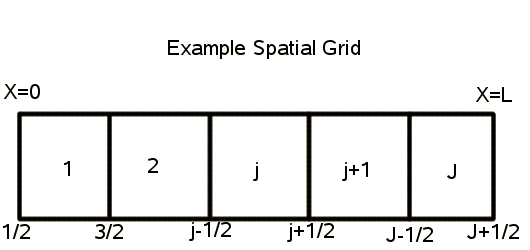
\includegraphics[width=\imgwidth,height=\imgheight]{SimpleGrid}}
		\end{picture}
		\caption{\label{fig:SimpleGrid} Simple one-dimensional orthogonal grid.}
		%\end{minipage} %\hfill
	\end{center}
\end{figure}

	The divergence of the flux in equation \ref{finalDiffusion} can be expressed as a simple edge centered differencing;
	\begin{equation}
	\label{dStream}
	\bar{\nabla}\cdot{F(\nu)}={F_{j+{1\over{2}}}(\nu)-F_{j-{1\over{2}}}(\nu)\over{\Delta{x_j}}}.
	\end{equation}
	The flux on either side of the cell edge can be written using Fick's law (equation \ref{FicksLaw});
	\begin{equation}
	\label{dStream2}
	F_{j+{1\over{2}}}^-(\nu)=-D_{j}(\nu){\left(E_{j+{1\over{2}}}(\nu)-E_j(\nu)\right)\over{{\Delta{x_{j}}\over{2}}}}
	\end{equation}
	and
	\begin{equation}
	\label{dStream3}
	F_{j+{1\over{2}}}^+(\nu)=-D_{j+1}(\nu){\left(E_{j+1}(\nu)-E_{j+{1\over{2}}}(\nu)\right)\over{{\Delta{x_{j+1}}\over{2}}}}.
	\end{equation}
	Finally, given the assumption that the flux is continuous it can be seen that
	\begin{equation}
	\label{dStream5}
	F_{j+{1\over{2}}}^+(\nu)=F_{j+{1\over{2}}}^-(\nu).
	\end{equation}
	The flux at the cell edge can now be written in terms of the cell centered energy density by combining equations \ref{dStream2} through \ref{dStream5}: 
	\begin{equation}
	\label{dStream6}
	F_{j+{1\over{2}}}(\nu)=-{2D_j(\nu)D_{j+1}(\nu)\over{\Delta{x_{j+1}}D_j(\nu)+\Delta{x_{j}}D_{j+1}(\nu)}}\left(E_{j+1}(\nu)-E_{j}(\nu)\right).
	\end{equation}
% 	Similarly, it can be shown that
% 	\begin{equation}
% 	\label{dStream7}
% 	F_{j-{1\over{2}}}(\nu)=-{2D_{j-1}(\nu)D_{j}(\nu)\over{\Delta{x_{j}}D_{j-1}(\nu)+\Delta{x_{j-1}}D_{j}(\nu)}}\left(E_{j}(\nu)-E_{j-1}(\nu)\right).
% 	\end{equation}
	With this new expressions for the photon flux at the cell edge the divergence of the flux becomes:
	\begin{eqnarray}
	\label{dStream8}
	&&\bar{\nabla}\cdot{F(\nu)}=-c{2D_j(\nu)D_{j+1}(\nu)\over{\Delta{x_j}\left(\Delta{x_{j+1}}D_j(\nu)+\Delta{x_{j}}D_{j+1}(\nu)\right)}}\left(E_{j+1}(\nu)-E_{j}(\nu)\right)\nonumber \\ & & +c{2D_{j-1}(\nu)D_{j}(\nu)\over{\Delta{x_j}\left(\Delta{x_{j}}D_{j-1}(\nu)+\Delta{x_{j-1}}D_{j}(\nu)\right)}}\left(E_{j}(\nu)-E_{j-1}(\nu)\right).
	\end{eqnarray}
	
	Inserting equation \ref{dStream8} into equation \ref{finalDiffusion} yields a tridiagonal system of equations for the cell centered energy density:
	\begin{equation}
	\label{disDiff}
	B_j(\nu)E_{j-1}^{t+1}(\nu) + D_j(\nu)E_j^{t+1}(\nu) + C_j(\nu)E_{j+1}^{t+1}(\nu) = Q^t_j(\nu),
	\end{equation}
	where
	\begin{equation}
	\label{distDiffB}
	B_j(\nu)=-{c2\Delta{t}D_{j-1}D_{j}\over{\Delta{x_j}\left(\Delta{x_{j}}D_{j-1}+\Delta{x_{j-1}}D_{j}\right)}},
	\end{equation}
	\begin{equation}
	\label{distDiffC}
	C_j(\nu)=-{c2\Delta{t}D_{j}(\nu)D_{j+1}(\nu)\over{\Delta{x_j}\left(\Delta{x_{j+1}}D_{j}(\nu)+\Delta{x_{j}}D_{j+1}(\nu)\right)}},
	\end{equation}
	\begin{equation}
	\label{distDiffD}
	D_j(\nu)=1+c\Delta{t}\sigma(\nu){f(T_j)}+c\Delta{t}\sigma(\nu){(1-f(T_j))} -A(\nu) -C(\nu), 
	\end{equation}
	and
	\begin{equation}
	\label{Q_j}
	Q_j(\nu)=c\Delta{t}\sigma_p(T_j)f(T_j)aT^4_j+c\Delta{t}{\sigma(\nu)b(\nu,T_j)\over{\sigma_p}}{\int{d\nu}E^{t+1}_j(\nu)\sigma_s(\nu)}+E_j(\nu).
	\end{equation}

\belowSubSecSkip

%==================%
% SubSubSection:   %
%    Energy Discretization %
%==================%
\subsubsection{Boundary Cells}
\label{sec:Transport-Discret-Boundary-Cells}

\noindent
	\indent There are two boundary conditions considered in this paper; an albedo boundary condition and an incident boundary flux. The albedo boundary condition can be described as a boundary that reflects some fraction($\gamma$) of the exiting boundary partial flux back into the boundary cell. The partial flux entering the right surface boundary can be expressed as 
	\begin{equation}
	\label{enteringPartialFlux}
	f_{{1\over{2}}}^-(\nu)={1\over{4}}E_{{1\over{2}}}(\nu)-{1\over{2}}F_{{1\over{2}}}(\nu),
	\end{equation}
	and the partial flux exiting the surface through the unit normal can be expressed as
	\begin{equation}
	\label{exitingPartialFlux}
	f_{{1\over{2}}}^+(\nu)={1\over{4}}E_{{1\over{2}}}(\nu)+{1\over{2}}F_{{1\over{2}}}(\nu).
	\end{equation}
	The total flux can be expressed as the difference of the partial flux incident on and exiting the left surface boundary.
	\begin{equation}
	\label{totalFlux}
	F_{{1\over{2}}}(\nu)={f_{{1\over{2}}}}^{-}(\nu)-{f_{{1\over{2}}}^+(\nu)}
	\end{equation}
	
	Given the case of an albedo boundary, the equation for the total flux (equation \ref{totalFlux}) becomes
	\begin{equation}
	\label{albedoTotalFlux}
	F_{{1\over{2}}}(\nu)=\gamma{f_{{1\over{2}}}}^{+}(\nu)-{f_{{1\over{2}}}^+(\nu)},
	\end{equation}
	where $\gamma$ denotes the precentage of the exiting flux that is reflected back into the system. Combining Fick's law, the partial fluxes, and the total flux (equation \ref{FicksLaw}, \ref{enteringPartialFlux}, \ref{exitingPartialFlux}, and \ref{albedoTotalFlux}) and solving for the left boundary flux in terms of $\gamma$ and $E_{j}(\nu)$ yields;
	\begin{equation}
	\label{albedoBoundar}
	F_{{1\over{2}}}(\nu)=-{2D_1(\nu)E_1(\nu)\left({1-\gamma\over{1+\gamma}}\right)\over{\Delta{x_1}\left(\left({1-\gamma\over{1+\gamma}}\right)+{4D_1(\nu)\over{\Delta{x}_1}}\right)}}.
	\end{equation}
	Similarly the flux for a right albedo boundary condition can be expressed as
	\begin{equation}
	\label{albedoBoundar}
	F_{J+{1\over{2}}}(\nu)={2D_J(\nu)E_J(\nu)\left({1-\gamma\over{1+\gamma}}\right)\over{\Delta{x_J}\left(\left({1-\gamma\over{1+\gamma}}\right)+{4D_J(\nu)\over{\Delta{x}}}\right)}}.
	\end{equation}

	For the case where the system has an incident flux on the left boundary, flux can be expressed as
	\begin{equation}
	\label{incidentPartialFlux}
	f_{{1\over{2}}}^-(\nu)={1\over{4}}E_{{1\over{2}}}(\nu)-{1\over{2}}F_{{1\over{2}}}(\nu)+F_o(\nu).
	\end{equation}
	Using this equation for the partial incident flux and the other equations used to solve the albedo boundary condition above results in the following expression for the total left boundary flux;
	\begin{equation}
	\label{incidentBoundaryCondition}
	F_{{1\over{2}}}(\nu)={2D_1(\nu)E_1(\nu)\left({4F_o(\nu)\over{c}}-E_1(\nu)\right)\over{\Delta{x_1}\left(1+{4D_1(\nu)\over{\Delta{x}_1}}\right)}}.
	\end{equation}
	Similarly the flux for a right incident flux boundary condition can be expressed as
	\begin{equation}
	\label{incidentBoundaryCondition}
	F_{J+{1\over{2}}}(\nu)=-{2D_J(\nu)E_J(\nu)\left({4F_o(\nu)\over{c}}-E_J(\nu)\right)\over{\Delta{x_J}\left(1+{4D_J(\nu)\over{\Delta{x}_J}}\right)}},
	\end{equation}
	where $F_o(\nu)$ denotes the incident partial flux.

\belowSubSecSkip

%=====================================================================%
% SubSection:                        	                              %
%     Transport: Summary %
%=====================================================================%
\subsection{Summary}
\label{sec:Transport-Summary}

\noindent
	\indent In this section the radiative transfer equation and material energy balance equation were transformed into an ``effective scattering'' diffusion equation. This diffusion equation was then discretized in space to generate a tridiagonal system for the cell-centered energy density at the next time step. Discretized forms of the boundary conditions were also derived

